\documentclass[10pt,letterpaper]{article}

% ---------- Page setup ----------
\usepackage[margin=0.68in]{geometry}
\usepackage[T1]{fontenc}
\usepackage[utf8]{inputenc}
\usepackage{lmodern}
\usepackage{microtype}
\usepackage{array}
\usepackage{booktabs}
\usepackage{tabularx}
\usepackage{longtable}
\usepackage{enumitem}
\usepackage{xcolor}
\usepackage{tikz}
\usepackage[most]{tcolorbox}
\usepackage{titlesec}
\usepackage{fancyhdr}
\usepackage{lastpage}
\usepackage[hidelinks]{hyperref}
\usepackage{ragged2e}
\usepackage{multicol}

% ---------- Colors ----------
\definecolor{Navy}{HTML}{17324D}
\definecolor{Blue}{HTML}{2563EB}
\definecolor{Teal}{HTML}{0F766E}
\definecolor{Green}{HTML}{15803D}
\definecolor{Amber}{HTML}{B45309}
\definecolor{Red}{HTML}{B91C1C}
\definecolor{Purple}{HTML}{6D28D9}
\definecolor{GrayText}{HTML}{475569}
\definecolor{LightBlue}{HTML}{EFF6FF}
\definecolor{LightTeal}{HTML}{ECFDF5}
\definecolor{LightAmber}{HTML}{FFFBEB}
\definecolor{LightGray}{HTML}{F8FAFC}
\definecolor{RuleGray}{HTML}{CBD5E1}

% ---------- Global formatting ----------
\setlength{\parindent}{0pt}
\setlength{\parskip}{4pt}
\renewcommand{\arraystretch}{1.2}
\setlength{\tabcolsep}{4pt}
\setlist[itemize]{leftmargin=*, nosep, topsep=2pt}
\setlist[enumerate]{leftmargin=*, nosep, topsep=2pt}
\titleformat{\section}{\Large\bfseries\color{Navy}}{}{0em}{}[\titlerule]
\titleformat{\subsection}{\large\bfseries\color{Navy}}{}{0em}{}
\titleformat{\subsubsection}{\normalsize\bfseries\color{Navy}}{}{0em}{}
\emergencystretch=2em
\sloppy

% ---------- Header/footer ----------
\pagestyle{fancy}
\fancyhf{}
\lhead{\textcolor{GrayText}{Enterprise AppSec and Operations Stack}}
\rhead{\textcolor{GrayText}{Handout}}
\cfoot{\textcolor{GrayText}{Page \thepage\ of \pageref{LastPage}}}
\renewcommand{\headrulewidth}{0.4pt}
\renewcommand{\footrulewidth}{0pt}

% ---------- Column types ----------
\newcolumntype{Y}{>{\RaggedRight\arraybackslash}X}
\newcolumntype{L}[1]{>{\RaggedRight\arraybackslash}p{#1}}

% ---------- Boxes ----------
\newtcolorbox{summarybox}{
  colback=LightBlue,
  colframe=Blue,
  boxrule=0.7pt,
  arc=2mm,
  left=8pt,
  right=8pt,
  top=7pt,
  bottom=7pt
}
\newtcolorbox{principlebox}{
  colback=LightTeal,
  colframe=Teal,
  boxrule=0.7pt,
  arc=2mm,
  left=8pt,
  right=8pt,
  top=7pt,
  bottom=7pt
}
\newtcolorbox{warningbox}{
  colback=LightAmber,
  colframe=Amber,
  boxrule=0.7pt,
  arc=2mm,
  left=8pt,
  right=8pt,
  top=7pt,
  bottom=7pt
}

\begin{document}

% ---------- Title ----------
{\Huge\bfseries\color{Navy} Enterprise AppSec and Operations Stack}\par
{\large\color{GrayText} A concise handout for tool roles, capability grouping, integration points, and governance usage}\par
\vspace{4pt}
{\small\color{GrayText} Prepared as a standalone architecture and planning reference.}\par
\vspace{10pt}

\begin{summarybox}
\textbf{Purpose.} This handout organizes a practical enterprise stack across application security testing, governance, IT operations, identity, training, project management, and customer management. The architecture is modular: each tool owns a clear capability, integrations exchange only decision-grade data, and identity should be centralized through Authentik wherever feasible.
\end{summarybox}

\begin{warningbox}
\textbf{Important licensing note.} Most tools in this stack are commonly deployed as open-source or open-source-centered platforms. GHAS, however, refers to GitHub Advanced Security and should be treated as a commercial GitHub security capability rather than an open-source SAST platform.
\end{warningbox}

\section{Tool Stack at a Glance}

\begin{longtable}{L{1.35in} L{1.05in} L{1.10in} L{3.10in}}
\toprule
\textbf{Capability Area} & \textbf{Tool} & \textbf{Primary Role} & \textbf{Enterprise Use Case} \\
\midrule
IAST & DongTai-IAST & Interactive Application Security Testing & Runtime vulnerability detection during functional testing, QA testing, or controlled integration environments. \\
SAST & GHAS & Static Application Security Testing & Code scanning, code security alerts, developer remediation workflows, and policy-driven review gates. \\
DAST & OWASP ZAP & Dynamic Application Security Testing & Web application scanning against deployed environments, API endpoints, and pre-production targets. \\
GRC & Eramba & Governance, Risk, and Compliance & Risk registers, policy mapping, control ownership, compliance tasks, and audit evidence tracking. \\
Project Management & Taiga & Agile Project Management & Product backlog, sprint planning, user stories, issue tracking, and delivery coordination. \\
ITAM & GLPI & IT Asset Management & Hardware, software, inventory, asset lifecycle, ownership, and support records. \\
ITSM & iTop & IT Service Management / CMDB & Incident, problem, change, service catalog, configuration items, dependency mapping, and operational workflows. \\
LMS & Moodle & Learning Management System & Security training, compliance courses, role-based learning paths, and training evidence. \\
Container Security & Trivy & Container and Dependency Scanner & Image scanning, software component inventory, vulnerability identification, and CI/CD security checks. \\
IAM & Authentik & Identity and Access Management & SSO, authentication, authorization integration, groups, application access, and identity federation. \\
CRM & SuiteCRM & Customer Relationship Management & Account management, customer communication, sales/service workflows, and stakeholder tracking. \\
\bottomrule
\end{longtable}

\section{Capability Grouping}

\begin{tabularx}{\textwidth}{L{1.65in} Y}
\toprule
\textbf{Layer} & \textbf{Tools and Role} \\
\midrule
Security Toolchain & DongTai-IAST, GHAS, OWASP ZAP, and Trivy provide layered application and infrastructure security testing across source code, running applications, deployed endpoints, containers, and dependencies. \\
Governance and Operations & Eramba, GLPI, and iTop provide risk governance, compliance tracking, asset management, service management, and configuration management. \\
Business Platforms & Taiga, Moodle, and SuiteCRM support delivery planning, training, customer/stakeholder workflows, and organizational enablement. \\
Identity Layer & Authentik should serve as the preferred identity control plane for SSO, authentication policy, group mapping, and application access governance. \\
\bottomrule
\end{tabularx}

\section{Reference Architecture View}

\begin{center}
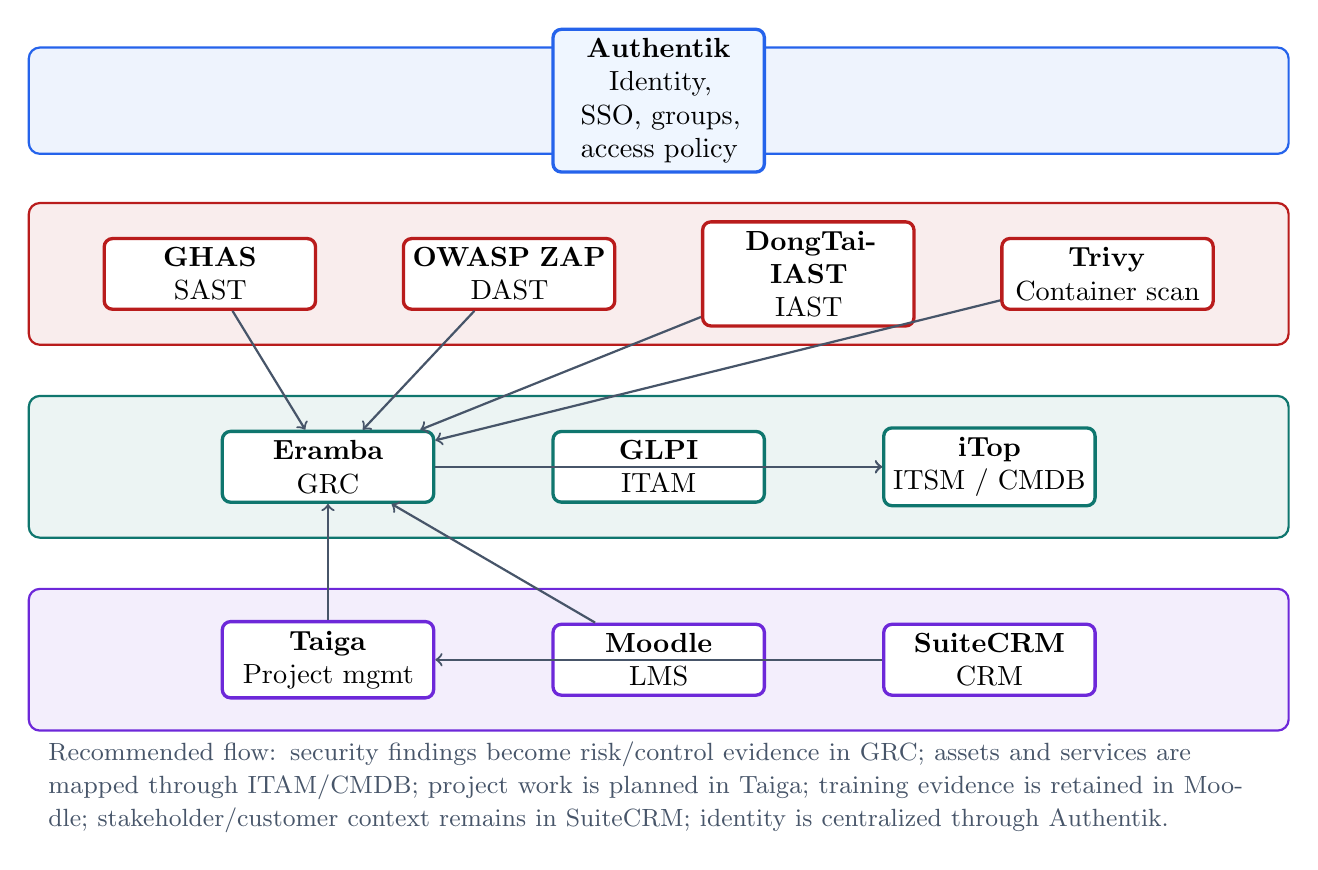
\begin{tikzpicture}[
  node distance=0.7cm,
  box/.style={rectangle, rounded corners=3pt, draw=RuleGray, very thick, align=center, minimum height=0.65cm, text width=2.45cm, fill=white},
  layer/.style={rectangle, rounded corners=4pt, draw=#1, thick, fill=#1!8, inner sep=8pt},
  arrow/.style={->, thick, draw=GrayText}
]

\node[layer=Blue, minimum width=16cm, minimum height=1.35cm] (identity) at (0,0) {};
\node[box, draw=Blue, fill=LightBlue] at (0,0) {\textbf{Authentik}\\Identity, SSO, groups, access policy};

\node[layer=Red, minimum width=16cm, minimum height=1.8cm] (security) at (0,-2.2) {};
\node[box, draw=Red] (ghas) at (-5.7,-2.2) {\textbf{GHAS}\\SAST};
\node[box, draw=Red] (zap) at (-1.9,-2.2) {\textbf{OWASP ZAP}\\DAST};
\node[box, draw=Red] (dongtai) at (1.9,-2.2) {\textbf{DongTai-IAST}\\IAST};
\node[box, draw=Red] (trivy) at (5.7,-2.2) {\textbf{Trivy}\\Container scan};

\node[layer=Teal, minimum width=16cm, minimum height=1.8cm] (govops) at (0,-4.65) {};
\node[box, draw=Teal] (eramba) at (-4.2,-4.65) {\textbf{Eramba}\\GRC};
\node[box, draw=Teal] (glpi) at (0,-4.65) {\textbf{GLPI}\\ITAM};
\node[box, draw=Teal] (itop) at (4.2,-4.65) {\textbf{iTop}\\ITSM / CMDB};

\node[layer=Purple, minimum width=16cm, minimum height=1.8cm] (business) at (0,-7.1) {};
\node[box, draw=Purple] (taiga) at (-4.2,-7.1) {\textbf{Taiga}\\Project mgmt};
\node[box, draw=Purple] (moodle) at (0,-7.1) {\textbf{Moodle}\\LMS};
\node[box, draw=Purple] (suitecrm) at (4.2,-7.1) {\textbf{SuiteCRM}\\CRM};

\draw[arrow] (ghas) -- (eramba);
\draw[arrow] (zap) -- (eramba);
\draw[arrow] (dongtai) -- (eramba);
\draw[arrow] (trivy) -- (eramba);
\draw[arrow] (eramba) -- (itop);
\draw[arrow] (glpi) -- (itop);
\draw[arrow] (taiga) -- (eramba);
\draw[arrow] (moodle) -- (eramba);
\draw[arrow] (suitecrm) -- (taiga);

\node[align=left, text width=15.5cm, color=GrayText] at (0,-8.72) {\small Recommended flow: security findings become risk/control evidence in GRC; assets and services are mapped through ITAM/CMDB; project work is planned in Taiga; training evidence is retained in Moodle; stakeholder/customer context remains in SuiteCRM; identity is centralized through Authentik.};
\end{tikzpicture}
\end{center}

\section{Security Testing Coverage Model}

\begin{tabularx}{\textwidth}{L{1.35in} L{1.15in} Y Y}
\toprule
\textbf{Testing Mode} & \textbf{Tool} & \textbf{Best Fit} & \textbf{Decision Output} \\
\midrule
SAST & GHAS & Pull requests, source repositories, code scanning rules, developer remediation loops. & Code security findings, severity, location, remediation status, approval or block decision. \\
DAST & OWASP ZAP & Running web applications, deployed test environments, API endpoints, and release validation. & Endpoint-level vulnerability findings, scan results, release risk evidence. \\
IAST & DongTai-IAST & Runtime instrumentation during QA or integration testing where application behavior can be observed. & Runtime vulnerability evidence, affected routes, data-flow context, exploitability signals. \\
Container / SCA & Trivy & Container images, operating system packages, application dependencies, and image promotion gates. & Vulnerability bill of materials, CVE list, severity threshold, pass/fail gate. \\
\bottomrule
\end{tabularx}

\section{Recommended Integration Principles}

\begin{principlebox}
\textbf{Design rule: integrate outcomes, not noise.} Avoid copying every raw scanner event into every platform. Send actionable, deduplicated, ownership-ready findings to governance and operations systems.
\end{principlebox}

\begin{enumerate}
  \item \textbf{Centralize identity first.} Use Authentik for SSO, group mapping, and application access control where supported.
  \item \textbf{Preserve system ownership boundaries.} Each platform should remain authoritative for its own domain: security testing, risk, assets, service operations, learning records, project delivery, or customer management.
  \item \textbf{Use GRC for accountability.} Eramba should track control ownership, risk acceptance, treatment plans, exceptions, audit evidence, and compliance obligations.
  \item \textbf{Use ITSM/CMDB for operational context.} iTop should connect incidents, changes, services, and configuration items to the systems affected by security or compliance events.
  \item \textbf{Use ITAM for inventory quality.} GLPI should maintain asset ownership, software inventory, hardware inventory, and lifecycle state.
  \item \textbf{Use project management for remediation delivery.} Taiga should track prioritized remediation stories, implementation tasks, release work, and sprint commitments.
  \item \textbf{Use LMS for evidence-backed training.} Moodle should retain training records for role-based security, compliance, and operational procedures.
\end{enumerate}

\section{Example End-to-End Workflow}

\begin{enumerate}
  \item Developer creates or updates code and submits work through the source-control workflow.
  \item GHAS performs SAST checks and identifies code-level security issues.
  \item Trivy scans container images and dependency components during build or promotion.
  \item OWASP ZAP tests deployed pre-production endpoints for dynamic web and API findings.
  \item DongTai-IAST observes runtime behavior during QA or integration testing.
  \item Validated findings are normalized, deduplicated, and linked to affected services or assets.
  \item Eramba records the risk, control relationship, exception status, owner, treatment plan, and evidence.
  \item iTop links the issue to the affected service, configuration item, change, or incident.
  \item GLPI provides asset ownership and lifecycle data when hardware or software inventory context is required.
  \item Taiga tracks remediation work as user stories, tasks, or defects.
  \item Moodle records required training or control-awareness completion when human process remediation is needed.
\end{enumerate}

\section{Governance Mapping}

\begin{tabularx}{\textwidth}{L{1.8in} Y Y}
\toprule
\textbf{Governance Question} & \textbf{Primary System} & \textbf{Supporting Systems} \\
\midrule
What risk exists? & Eramba & GHAS, OWASP ZAP, DongTai-IAST, Trivy \\
Which service or asset is affected? & iTop / GLPI & Eramba, Authentik \\
Who owns remediation? & Taiga & iTop, GLPI, Eramba \\
Who has access? & Authentik & iTop, GLPI, Eramba \\
What evidence proves control operation? & Eramba & Moodle, GHAS, Trivy, ZAP, DongTai-IAST \\
Who completed required training? & Moodle & Authentik, Eramba \\
Which customer or stakeholder is impacted? & SuiteCRM & Taiga, iTop \\
\bottomrule
\end{tabularx}

\section{Implementation Checklist}

\begin{multicols}{2}
\begin{itemize}
  \item Define authoritative ownership for each platform.
  \item Establish Authentik SSO and group strategy.
  \item Define severity thresholds for GHAS, ZAP, DongTai-IAST, and Trivy.
  \item Normalize scanner output into a common finding model.
  \item Map applications to services, assets, owners, and business context.
  \item Create Eramba risk and control workflows.
  \item Create iTop service and CMDB relationships.
  \item Create GLPI asset ownership and lifecycle rules.
  \item Create Taiga remediation templates and priorities.
  \item Create Moodle training tracks for security and compliance roles.
  \item Define exception, risk acceptance, and waiver processes.
  \item Establish reporting for open risk, SLA status, remediation progress, and training completion.
\end{itemize}
\end{multicols}

\section{Operating Model Summary}

\begin{tabularx}{\textwidth}{L{1.55in} Y}
\toprule
\textbf{Operating Principle} & \textbf{Practical Meaning} \\
\midrule
Clear ownership & Every finding, asset, service, project task, risk, and training requirement should have an accountable owner. \\
Layered testing & SAST, DAST, IAST, and container scanning should be complementary controls, not competing tools. \\
Evidence-driven governance & Compliance reporting should be based on retained evidence, not manual status claims. \\
Operational traceability & Security issues should be traceable from source finding to affected service, risk record, remediation task, and closure evidence. \\
Centralized access control & Identity, SSO, and access groups should be managed consistently through Authentik wherever technically feasible. \\
\bottomrule
\end{tabularx}

\vfill
\begin{center}
{\small\color{GrayText} End of handout}
\end{center}

\end{document}
